% \chapter{Title of the Experiment}


=-\chapter{Equivalent spring constant of combination of springs}

Date: 14/9/2020

% Date: 5/9/2020

\section{Aim}

In this experiment, our aim is to calculate the equivalent spring constant of combination of springs, in both series and parallel. We derive the relationship of spring constant by applying varying weight on springs in series and parallel.


\section{Background Theory}

Hooke's Law states force applied on a spring is proportional to its extension, given its limit of proportionality has not reached. Mathematically, it can be expressed as $$ F= k \Delta x $$ where F is force applied, k denotes spring constant and $\Delta x$ is change in length of spring. When the spring reaches its elastic limit then it can not return back to its original shape and is deformed. 
When the springs are attached in series, the extension is equal to
    $$ \Delta x = \Delta x_1 + \Delta x_2 $$
The force that is applied  on both the strings is same, consequently :
    $$ F = k(\Delta x_1 + \Delta x_2) $$
    $$ F = k_1 \Delta x_1 $$
    $$ F = k_2 \Delta x_2 $$
We can then combine these equations to get an expression for k, there combined spring constant.
    $$ k_1 \Delta x_1 =  k_2 \Delta x_2 $$
    $$ \Delta x_2 = \frac{K_1 \Delta x_1}{k_2} $$
    $$ F = k(\Delta x_1 + \frac{K_1 \Delta x_1}{k_2}) $$ 
    $$ F = k(1 + \frac{k1}{k2}) \Delta x_1 $$
    $$ k_1 \Delta x_1 = k(1 + \frac{k1}{k2}) \Delta x_1 $$
    $$ k = \frac{k_1 \times k_2}{k_1 +k_2} $$
When springs are attached in parallel, the total force is equal to
    $$ F = F_1 + F_2 $$
The extension of both the springs is same, Consequently:
    $$ F = k \Delta x $$
    $$ F_1 = k_1 \Delta x $$
    $$ F_2 = k_2 \Delta x $$
We can then combine these equations to get an expression for k,
there combined spring constant.

$$ k \Delta x = k_1 \Delta x + k_2 \Delta x $$
$$ k \Delta x = \Delta x( k_1 + k_2) $$
$$ k = k_1 + k_2 $$




% \begin{figure}[htbp]
% \centerline{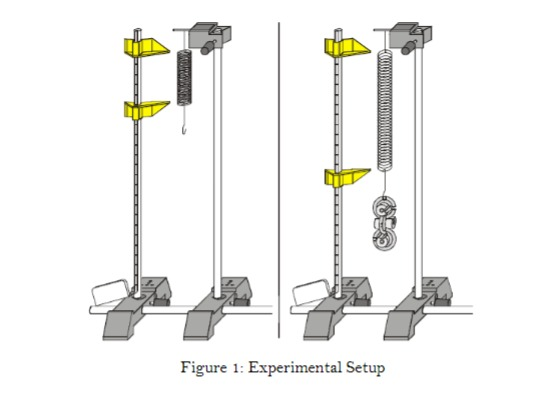
\includegraphics[width=3in, height=2in]{figures/fig3.jpeg}}
% \caption{This is an image from a text that uses color to teach music.}
% % \label{fig}
% \end{figure}

% \begin{figure}[h!]
%     \centering
%     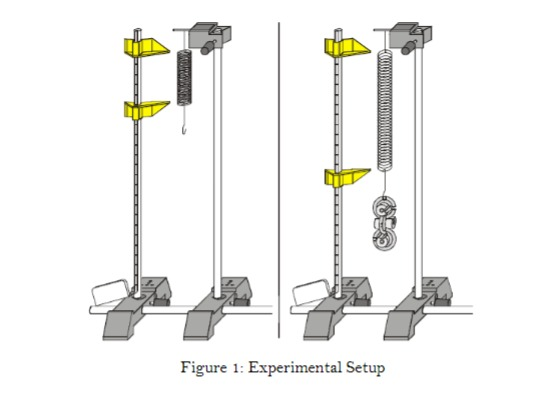
\includegraphics[width=\textwidth]{figures/fig3.jpeg}
%     \caption{Apparatus}
%     \label{fig:yx}
% \end{figure}
\section{Description of Setup}
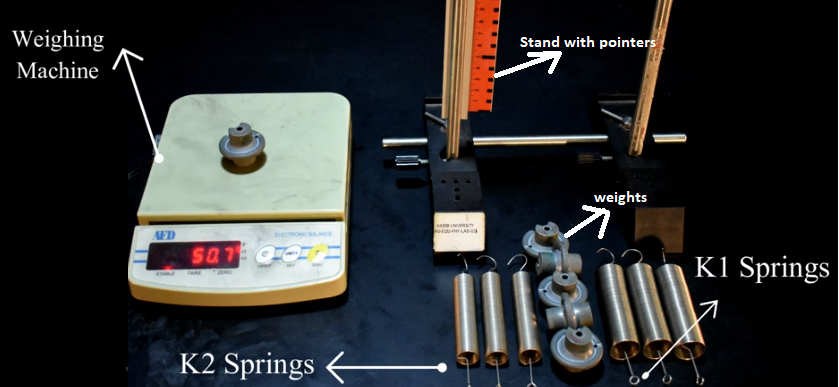
\includegraphics[width=12cm, height=7cm]{figures/fig1.png} \\
Here the stand with pointers gives easy access to measuring the length and spring is supported on a clamp.The weights are then suspended from the spring.

\section{Method / Procedure}
The initial length of the spring is measured using the pointer stand and weights are suspended and the springs length is measured. This is repeated with adding more weights and change in the length of spring is measured. 
This is carried out for setting up the springs in series and parallel. 
The springs constant is calculated using Hooke's law by determining slope of the graph of extension against weight of masses.

\section{Data}

In this experiment, since the mass of the weights and the extension in length is measured only once they don't not have type A uncertainty. The type B certainty associated with the length and mass is respectively 0.0002m and 0.03g

\begin{center}
    
\begin{tabular}{|c|c|c|c|c|}
\hline
\multicolumn{5}{|c|}{\textbf{Initial Measurements}}                     \\ \hline
Springs & dia   (cm) & single   (cm) & series   (cm) & parallel   (cm) \\ \hline
K1      & 2.051      & 7.7           & 22.9          & 7.7             \\ \hline
K2      & 1.524      & 7.7           & 20.3          & 7.7             \\ \hline
K1+K2   & -          & -             & 21.9          & 7.7             \\ \hline
\end{tabular}
\end{center}

\begin{center}
\begin{tabular}{|c|c|c|c|c|c|}
\hline
\multicolumn{6}{|c|}{\textbf{K1 (single)}}                                          \\ \hline
s.No & Mass   (grams) & Upper   (cm) & Lower   (cm) & Diff     (cm) & Ext      (cm) \\ \hline
1    & 0              & 94.2         & 86.5         & 7.7           & 0             \\ \hline
2    & 50.7           & 94.2         & 81.9         & 12.3          & 4.6           \\ \hline
3    & 101.4          & 94.2         & 77.2         & 17            & 9.3           \\ \hline
4    & 152.1          & 94.2         & 72.7         & 21.5          & 13.8          \\ \hline
5    & 202.8          & 94.2         & 68.1         & 26.1          & 18.4          \\ \hline
6    & 253.5          & 94.2         & 63.6         & 30.6          & 22.9          \\ \hline
7    & 304.2          & 94.2         & 58.3         & 35.9          & 28.2          \\ \hline
\end{tabular}
\end{center}

\begin{center}
\begin{tabular}{|c|c|c|c|c|c|}
\hline
\multicolumn{6}{|c|}{\textbf{K1 (series)}}                                          \\ \hline
s.No & Mass   (grams) & Upper   (cm) & Lower   (cm) & Diff     (cm) & Ext      (cm) \\ \hline
1    & 0              & 94.2         & 71.3         & 22.9          & 0             \\ \hline
2    & 50.7           & 94.2         & 62.6         & 31.6          & 8.7           \\ \hline
3    & 101.4          & 94.2         & 53.1         & 41.1          & 18.2          \\ \hline
4    & 152.1          & 94.2         & 43.6         & 50.6          & 27.7          \\ \hline
5    & 202.8          & 94.2         & 34.2         & 60            & 37.1          \\ \hline
6    & 253.5          & 94.2         & 25           & 69.2          & 46.3          \\ \hline
7    & 304.2          & 94.2         & 15.7         & 78.5          & 55.6          \\ \hline
\end{tabular}
\end{center}

\begin{center}
\begin{tabular}{|c|c|c|c|c|c|}
\hline
\multicolumn{6}{|c|}{\textbf{K1 (parallel)}}                                        \\ \hline
s.No & Mass   (grams) & Upper   (cm) & Lower   (cm) & Diff     (cm) & Ext      (cm) \\ \hline
1    & 0              & 94.2         & 86.5         & 7.7           & 0             \\ \hline
2    & 50.7           & 94.2         & 84           & 10.2          & 2.5           \\ \hline
3    & 101.4          & 94.2         & 81.7         & 12.5          & 4.8           \\ \hline
4    & 152.1          & 94.2         & 79.2         & 15            & 7.3           \\ \hline
5    & 202.8          & 94.2         & 77.2         & 17            & 9.3           \\ \hline
6    & 253.5          & 94.2         & 74.7         & 19.5          & 11.8          \\ \hline
7    & 304.2          & 94.2         & 72.3         & 21.9          & 14.2          \\ \hline
\end{tabular}
\end{center}

\begin{center}
\begin{tabular}{|c|c|c|c|c|c|}
\hline
\multicolumn{6}{|c|}{\textbf{K2 (single)}}                  \\ \hline
s.No & Mass   (grams) & l1   & l2   & final & Ext      (cm) \\ \hline
1    & 0              & 94.2 & 86.5 & 7.7   & 0             \\ \hline
2    & 50.7           & 94.2 & 84.9 & 9.3   & 1.6           \\ \hline
3    & 101.4          & 94.2 & 82.8 & 11.4  & 3.7           \\ \hline
4    & 152.1          & 94.2 & 81   & 13.2  & 5.5           \\ \hline
5    & 202.8          & 94.2 & 79.1 & 15.1  & 7.4           \\ \hline
6    & 253.5          & 94.2 & 77.4 & 16.8  & 9.1           \\ \hline
7    & 304.2          & 94.2 & 75.6 & 18.6  & 10.9          \\ \hline
\end{tabular}
\end{center}

\begin{center}
    
\begin{tabular}{|c|c|c|c|c|c|}
\hline
\multicolumn{6}{|c|}{\textbf{K1 and K2 (series)}}                                   \\ \hline
s.No & Mass   (grams) & Upper   (cm) & Lower   (cm) & Diff     (cm) & Ext      (cm) \\ \hline
1    & 0              & 94.2         & 72.3         & 21.9          & 0             \\ \hline
2    & 50.7           & 94.2         & 65.8         & 28.4          & 6.5           \\ \hline
3    & 101.4          & 94.2         & 59.4         & 34.8          & 12.9          \\ \hline
4    & 152.1          & 94.2         & 52.5         & 41.7          & 19.8          \\ \hline
5    & 202.8          & 94.2         & 46.2         & 48            & 26.1          \\ \hline
6    & 253.5          & 94.2         & 39.5         & 54.7          & 32.8          \\ \hline
7    & 304.2          & 94.2         & 33           & 61.2          & 39.3          \\ \hline
\end{tabular}
\end{center}


\begin{center}
\begin{tabular}{|c|c|c|c|c|c|}
\hline
\multicolumn{6}{|c|}{\textbf{K1 and K2 (series)}}                                   \\ \hline
s.No & Mass   (grams) & Upper   (cm) & Lower   (cm) & Diff     (cm) & Ext      (cm) \\ \hline
1    & 0              & 94.2         & 72.3         & 21.9          & 0             \\ \hline
2    & 50.7           & 94.2         & 65.8         & 28.4          & 6.5           \\ \hline
3    & 101.4          & 94.2         & 59.4         & 34.8          & 12.9          \\ \hline
4    & 152.1          & 94.2         & 52.5         & 41.7          & 19.8          \\ \hline
5    & 202.8          & 94.2         & 46.2         & 48            & 26.1          \\ \hline
6    & 253.5          & 94.2         & 39.5         & 54.7          & 32.8          \\ \hline
7    & 304.2          & 94.2         & 33           & 61.2          & 39.3          \\ \hline
\end{tabular}
\end{center}


\section{Data Analysis}
\begin{center}
\begin{figure}[h!]
    \centering
    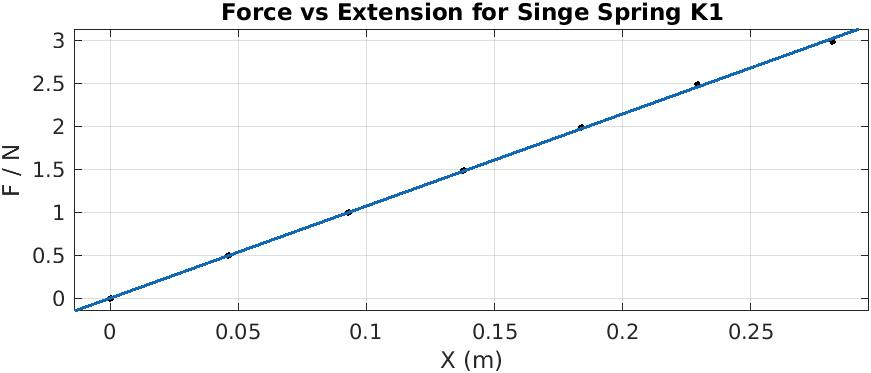
\includegraphics[width=\textwidth]{figures/K1.jpg}
    \caption{Graph of Force vs Extension for spring K1}
    \label{fig:k1}
\end{figure}
\end{center}


$$ K1_{single} = 10.72 N/m $$

\newpage
\begin{center}
\begin{figure}[h!]
    \centering
    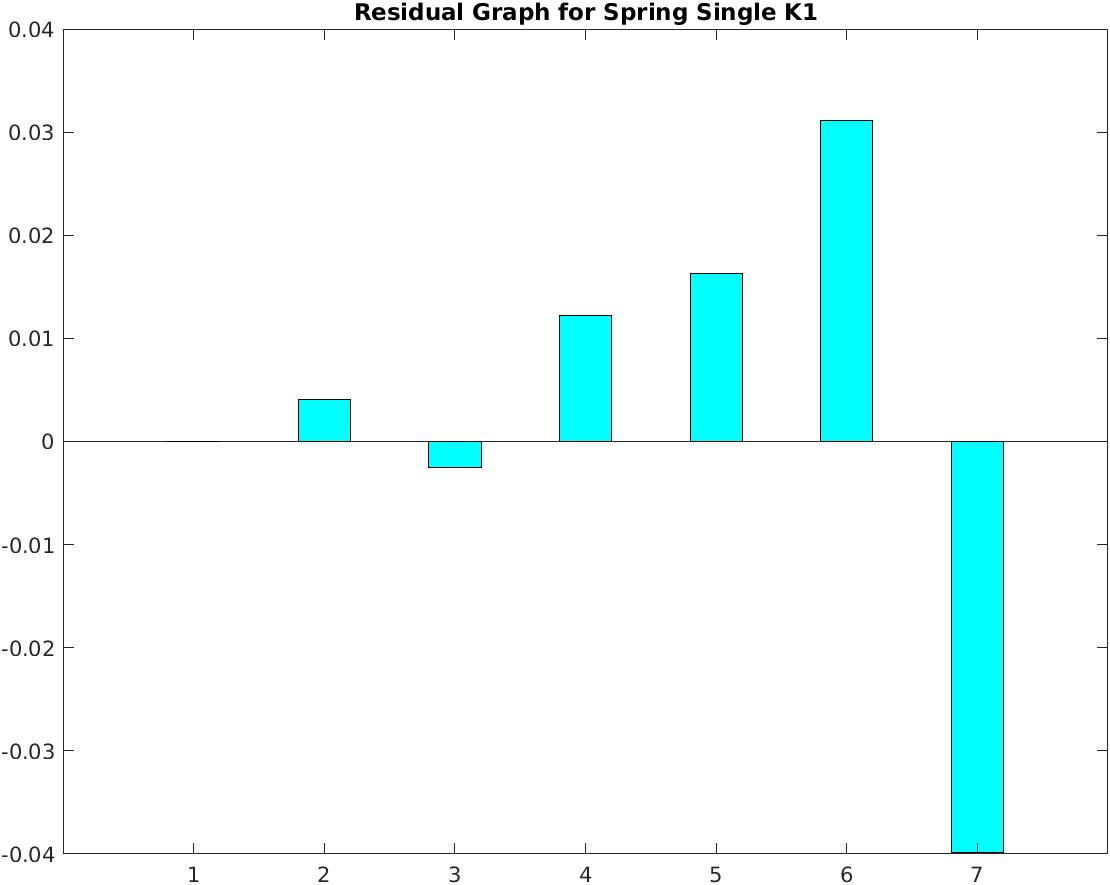
\includegraphics[width=\textwidth]{figures/K1_S_R.jpg}
    \caption{Residual Plot for Single Spring K1}
    \label{fig:k1_S_R}
\end{figure}
\end{center}

\begin{center}
\begin{figure}[h!]
    \centering
    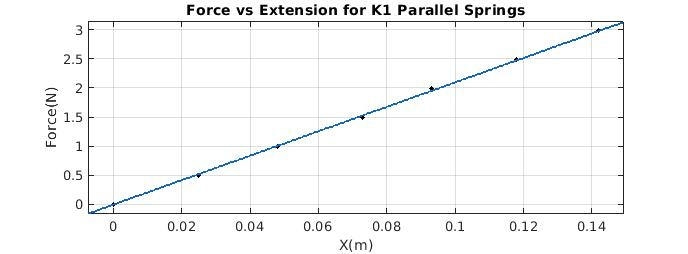
\includegraphics[width=\textwidth]{figures/K1_P.jpg}
    \caption{Graph of Force vs Extension for K1 Parallel Springs}
    \label{fig:k1_P}
\end{figure}
\end{center}
$$ K1_{Parallel} = 21 N/m $$
\newpage
\begin{center}
\begin{figure}[h!]
    \centering
    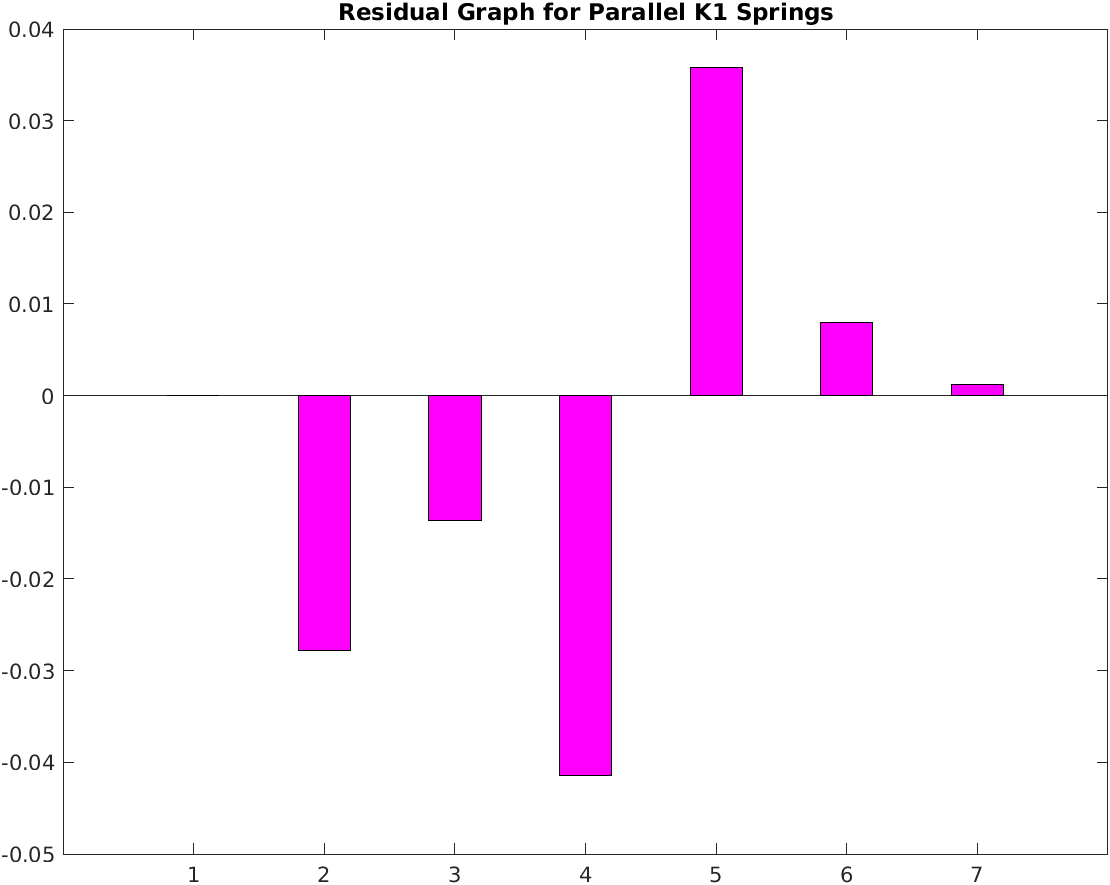
\includegraphics[width=\textwidth]{figures/K1_P_R.png}
    \caption{Residual Plot for Single K1 Parallel Springs}
    \label{fig:k1_P_R}
\end{figure}
\end{center}

\begin{center}
\begin{figure}[h!]
    \centering
    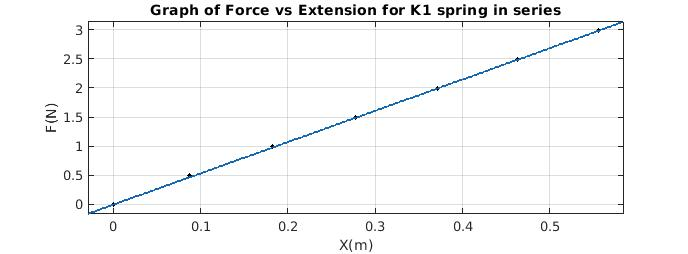
\includegraphics[width=\textwidth]{figures/K1_S_se.jpg}
    \caption{Graph of Force vs Extension for K1 Springs in Series}
    \label{fig:k1_S_se}
\end{figure}
\end{center}
$$ K1_{Parallel} = 5.375 N/m $$
\newpage
\begin{center}
\begin{figure}[h!]
    \centering
    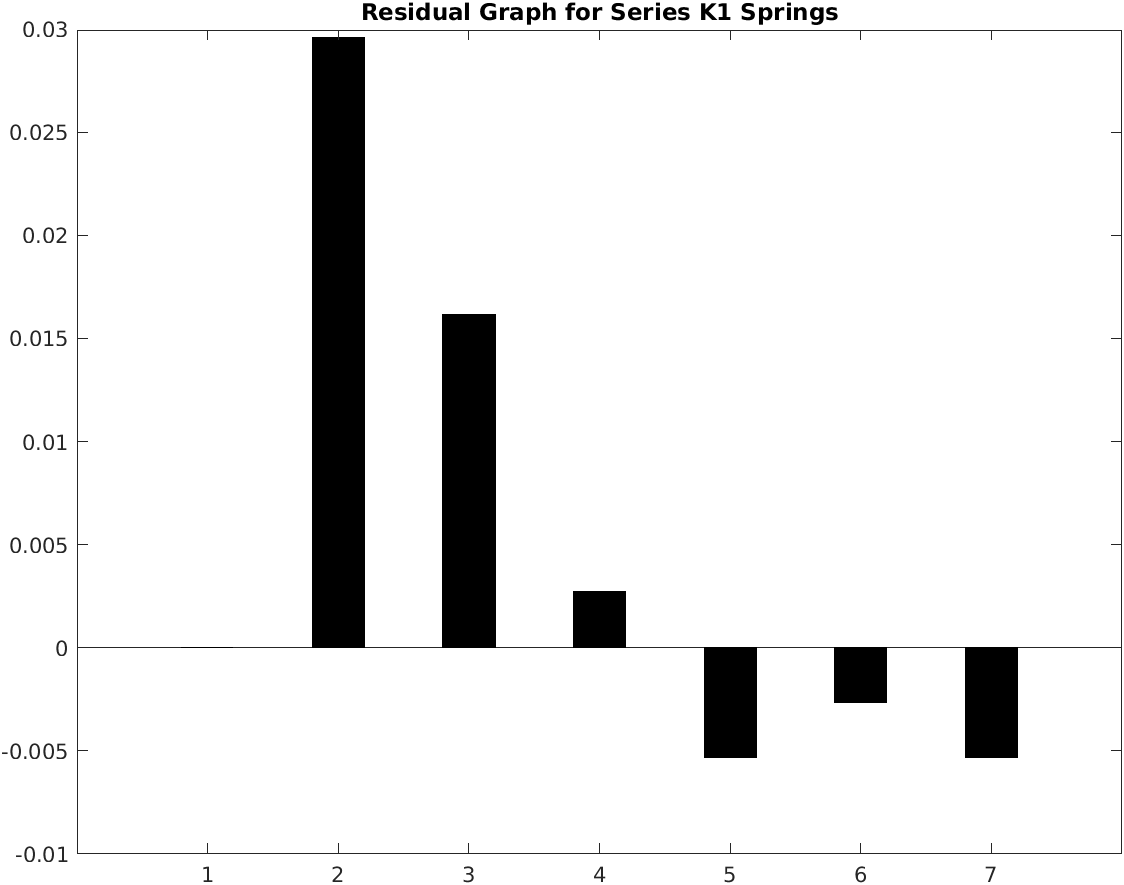
\includegraphics[width=\textwidth]{figures/K1_Se_R.png}
    \caption{Residual Plot for K1 Springs in Series}
    \label{fig:k1_Se_R}
\end{figure}
\end{center}

%%% K2 Single

\begin{center}
\begin{figure}[h!]
    \centering
    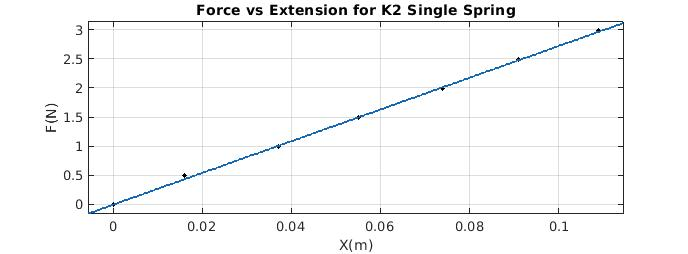
\includegraphics[width=\textwidth]{figures/K2_Single.jpg}
    \caption{Graph of Force vs Extension for Single Spring K2}
    \label{fig:k1_Se_R}
\end{figure}
\end{center}

$$ K2_{single} = 27.25 N/m $$

\newpage
\begin{center}
\begin{figure}[h!]
    \centering
    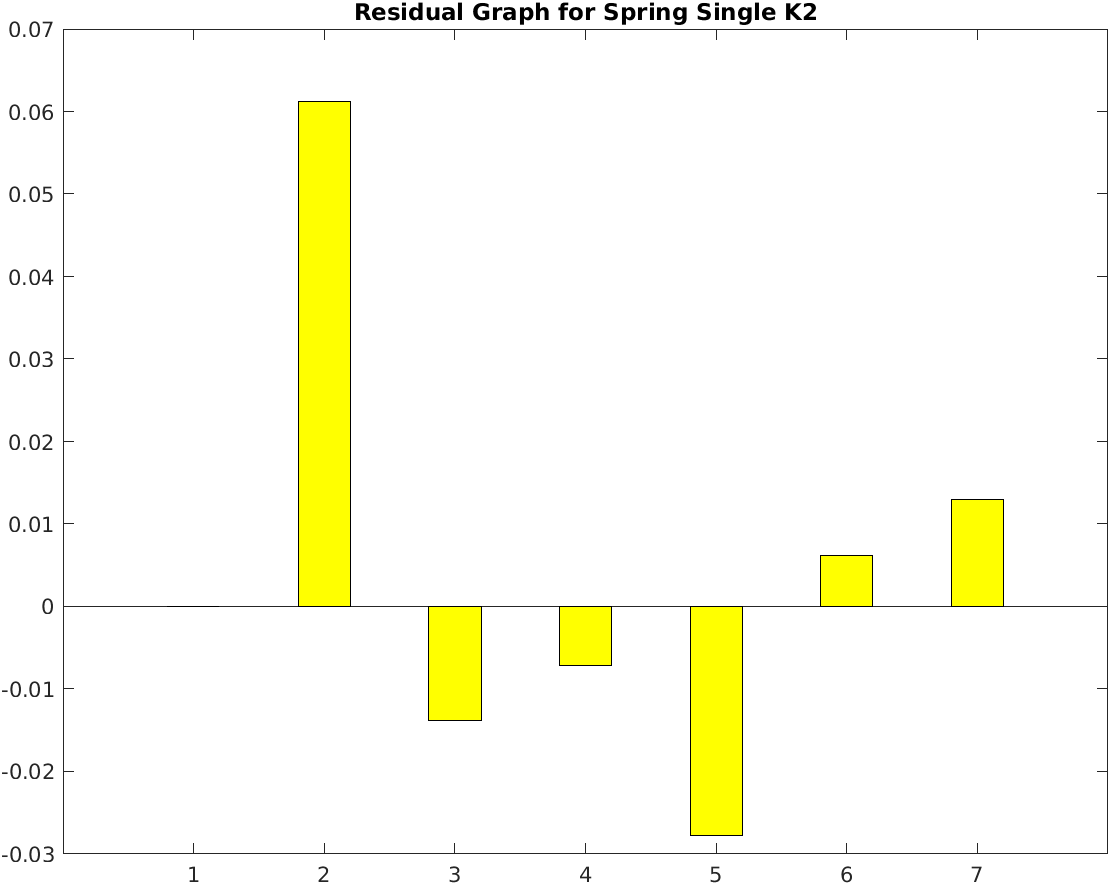
\includegraphics[width=\textwidth]{figures/k2_single.png}
    \caption{Residual Plot for Single K2 Spring}
    \label{fig:k1_Se_R}
\end{figure}
\end{center}

%%%% K2 Series

\begin{center}
\begin{figure}[h!]
    \centering
    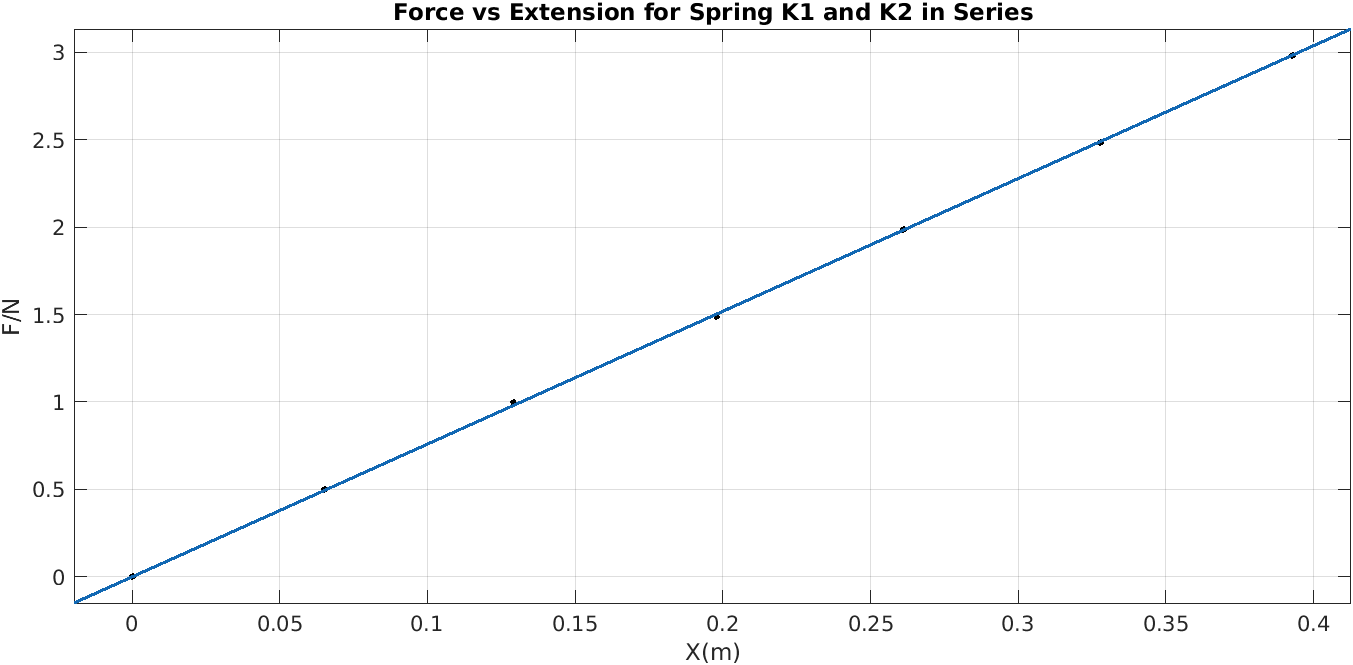
\includegraphics[width=\textwidth]{figures/k1_k2_ser.png}
    \caption{Graph of Force vs Extension for Spring K1 and K2 in series}
    \label{fig:k1_Se_R}
\end{figure}
\end{center}

$$ {K1 and K2}_{series} = 7.593 N/m $$

\begin{center}
\begin{figure}[h!]
    \centering
    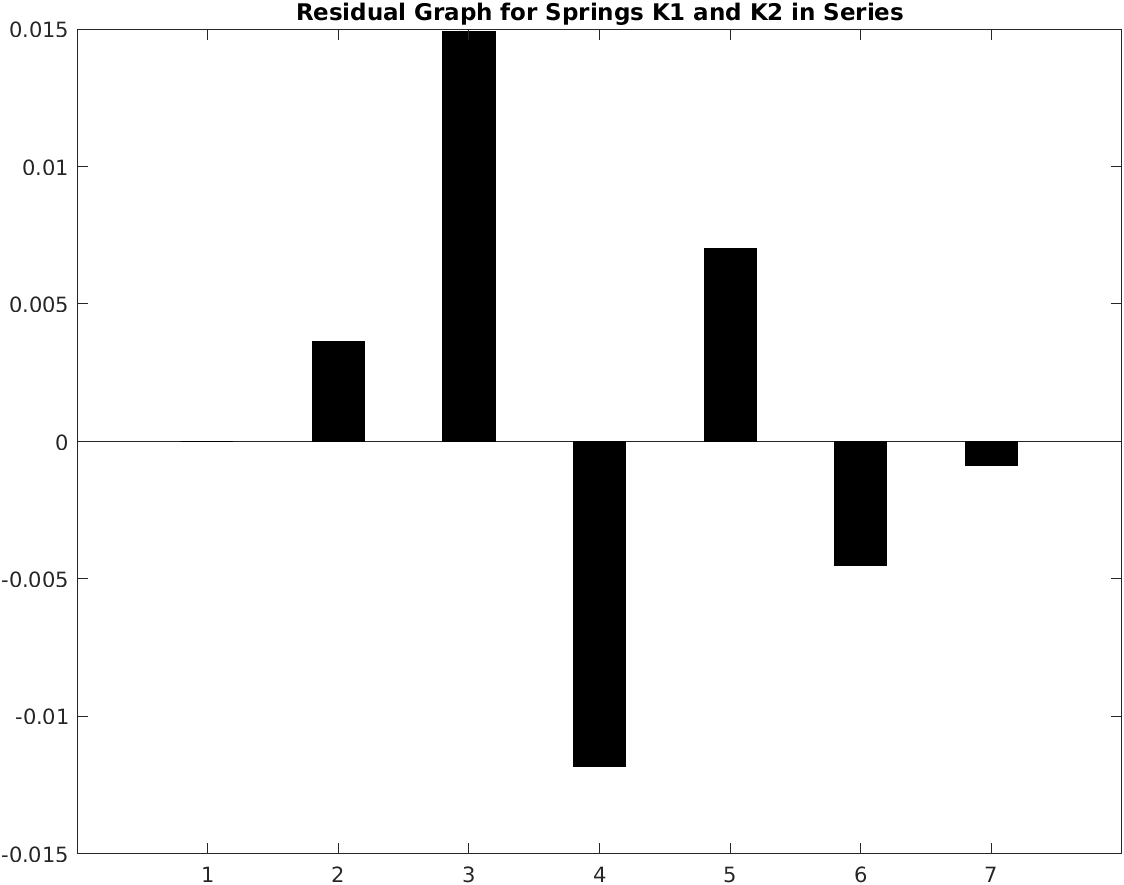
\includegraphics[width=\textwidth]{figures/K1_K2_Series_R.png}
    \caption{Residual Plot for Parallel Springs K1 and K2 in Series}
    \label{fig:k1_Se_R}
\end{figure}
\end{center}

%%%% K2 Parallel
\newpage
\begin{center}
\begin{figure}[h!]
    \centering
    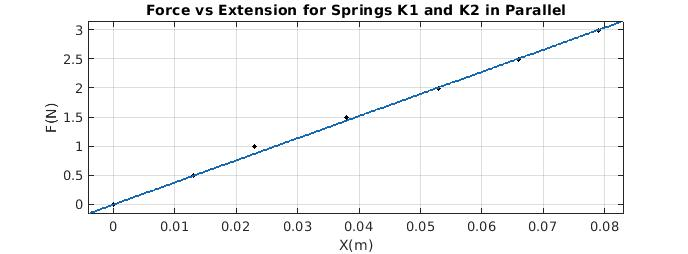
\includegraphics[width=\textwidth]{figures/K1_K2_Parallel.jpg}
    \caption{Graph of Force vs Extension for Springs K1 and K2 in Parallel}
    \label{fig:k1_Se_R}
\end{figure}
\end{center}

$$ {K1 and K2}_{Parallel} = 38.02 N/m $$


\begin{center}
\begin{figure}[h!]
    \centering
    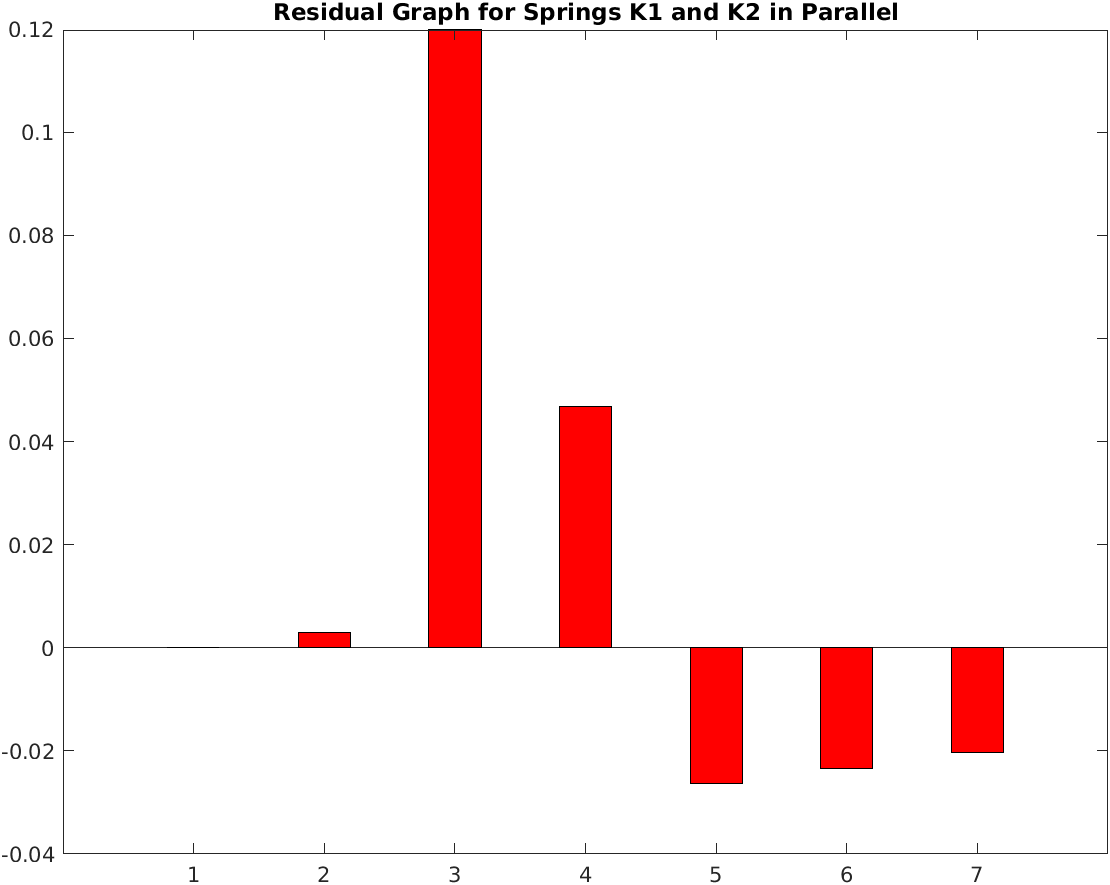
\includegraphics[width=\textwidth]{figures/K1_K2_Parallel_R.png}
    \caption{Residual Plot for Parallel Springs K1 and K2 in Parallel}
    \label{fig:k1_Se_R}
\end{figure}
\end{center}
Theoretical value of K1 and K2 in series = $ 7.695 N/m$ \\
Theoretical value of K1 and K2 in Parallel = $ 37.97 N/m$ \\

\section{Discussion \& Conclusion}
The theoretical and experimental values are the following: 7.593 experimental and 7.695 is experimental values of spring constant for series, they have an error of 0.1 which is quite small. For parallel experimental value is 38.02 and theoretical is 37.97, with error of 0.05. We can also see the random pattern in the residual plots that indicate random errors. Our experimental values are closely matching with theoretical values so our hypothesis is supported by this experiment. \\
 Possible factors of uncertainty and errors can be varying shape of spring, if we attach weights that exceed the springs the springs elastic limit then the spring can deform.
 
 

% Summarize and discuss the experimental results, what do the results say about your hypothesis, if such a hypothesis was made for the experiment. Mention the uncertainty in the calculated quantity Be precise and only include scientific discussion.


\section{MATLAB Script}
\lstinputlisting{matlabCodes/Experiment2.m}



